\chapter{Data Analysis and Processing}

\section{ Data Description}
The first figure below shows the structure of the dataset where all attributes are shown, with 
their type, in addition to a glimpse of the variables within each Attribute; as shown at the end of 
the figure, the Class type is integer, which I needed to change to factor and identify the 0 as Not 
Fraud and the one as Fraud to ease the process of creating the modeland obtain visualizations.The second figure shows the class distribution; the red bar, which contains 284,315variables, 
represents the non-fraudulent transactions, and the blue bar, with 492 variables, represents the 
fraudulent transactions.

\begin{figure}[h]
   \centering
   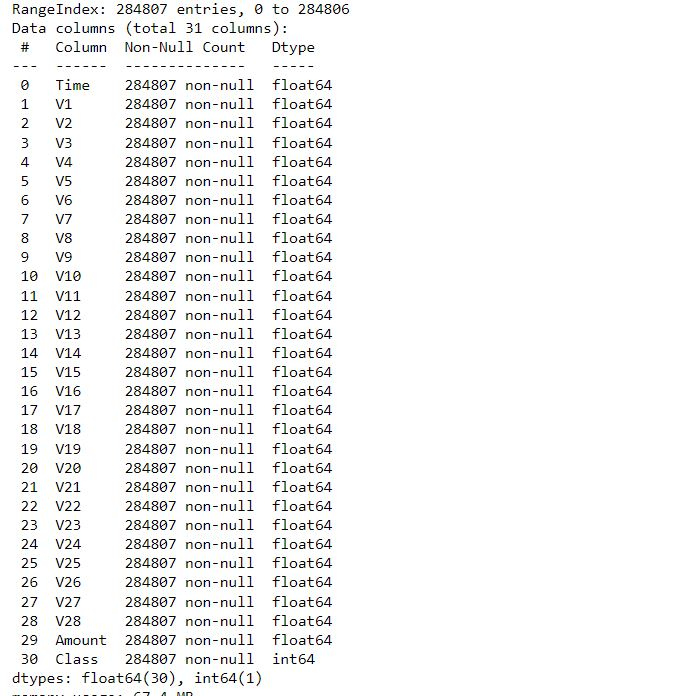
\includegraphics[width=5.5in]{Chap4/Data Structure.JPG}
   \caption{Data Structure}
   \label{fig:Data Structure}
\end{figure}

\begin{figure}[h]
   \centering
   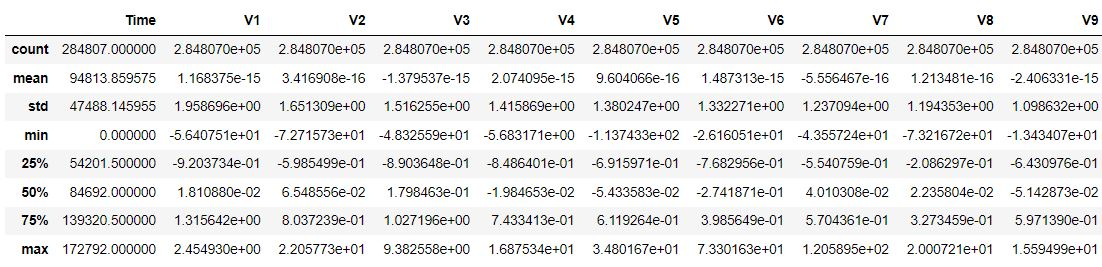
\includegraphics[width=5.5in]{Chap4/Data description.JPG}
   \caption{Data Description}
   \label{fig:Data Description}
\end{figure}

\begin{figure}[h]
   \centering
   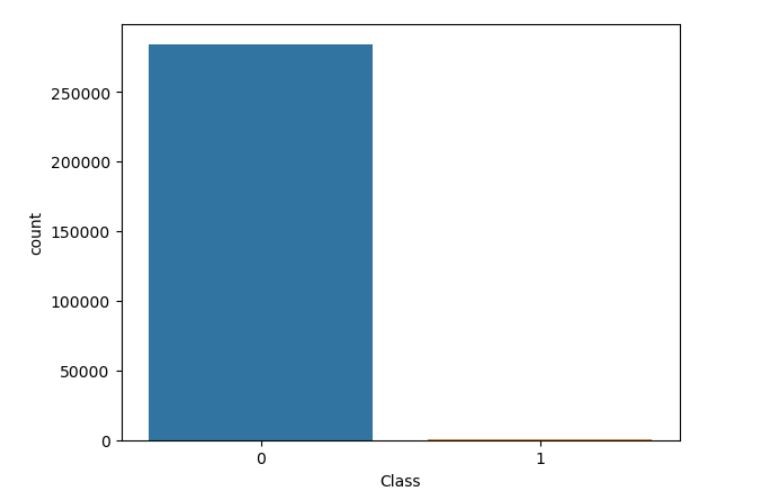
\includegraphics[width=5.5in]{Chap4/Count Class-Data.JPG}
   \caption{Class Count}
   \label{fig:Class Count}
\end{figure}


\section{ Analysis }

\begin{figure}[h]
   \centering
   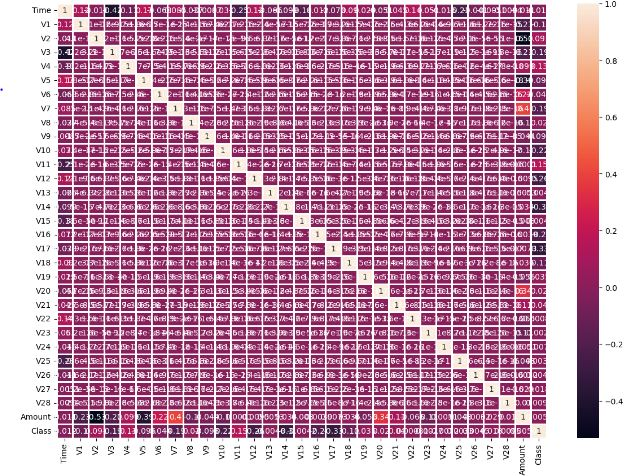
\includegraphics[width=5.5in]{Chap4/Data Corelation.JPG}
   \caption{Data Correlation}
   \label{fig:Data Correlation}
\end{figure}

\begin{figure}[h]
   \centering
   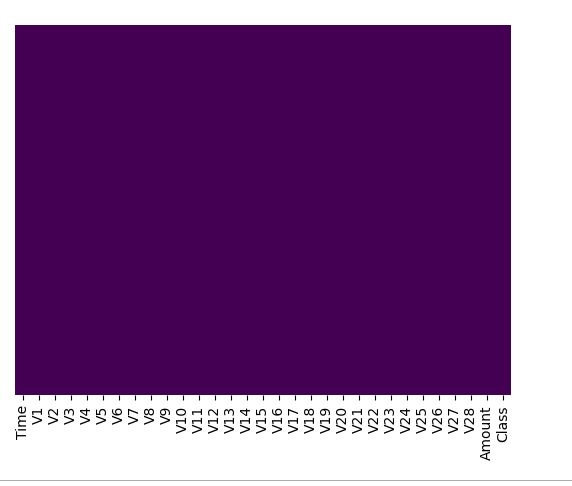
\includegraphics[width=5.5in]{Chap4/Check_Null_data.JPG}
   \caption{Null data}
   \label{fig:Checking Null data}
\end{figure}




